% !TeX root = Thesis.tex
\chapter{The Barcode of a Non-Autonomous Hamiltonian}

In this chapter we compute the barcode of a specific non-autonomous Hamiltonian on the torus. This requires computing the contractible periodic orbits of this Hamiltonian, computing their Maslov indices, and computing their differentials. To compute the contractible periodic orbits, we will apply a trick based on covering spaces. To compute their Maslov indices, we apply the tools developed in chapter \ref{chap:maslov}. Finally, to compute the differentials we will apply a trick based on symmetry of the space and the Hamiltonian of study.

\section{The Hamiltonian}

Let $M = S^1 \times S^1$ be the torus with the usual symplectic structure $\dl x \wedge \dl y$, where $x$ and $y$ are the coordinates in each $S^1$, with period $2\pi$.

In order to construct a Hamiltonian diffeomorphism suitable for study, we begin by exhibiting a simple class of such diffeomorphisms.

\begin{lemma}
Let $f \colon S^1 \to \R$ be a smooth function with null mean. Then, the map
\begin{equation}
\phi_f(x,y) = (x, y + f(x)),
\end{equation}
is a Hamiltonian diffeomorphism. It is generated by the Hamiltonian
\begin{equation}
H(x,y) = \int_0^x f(t) \dl3 t,
\end{equation}
whose time-$t$ flow is given by
\begin{equation}
\phi_{tf}(x,y) = (x, y + t f(x)).
\end{equation}
\end{lemma}

\begin{proof}
The exhibited Hamiltonian has differential given by
\begin{equation}
\dl H = f(x) \dl x,
\end{equation}
which satisfies
\begin{equation}
\dl H = - (f(x) \partial_y) \into (\dl x \wedge \dl y),
\end{equation}
hence $X^H = f(x) \partial_y$, whose time-$t$ flow is clearly $\phi_{tf}$.
\end{proof}

The same can be done in the other coordinate, yielding a Hamiltonian diffeomorphism of the form $(x,y) \mapsto (x + g(y), y)$. It is a classical result that the Hamiltonian diffeomorphisms are closed under composition, and hence we may construct a Hamiltonian diffeomorphism
\begin{equation}
(x,y) \mapsto (x + g(y+f(x)), y+f(x)).
\end{equation}

We define our object of study as the particular case when $f = g = a \sin$, where $a$ is a real parameter, yielding the Hamiltonian diffeomorphism
\begin{equation}\label{eq:phi1def}
\phi(x,y) = ( x + a \sin(y + a \sin(x)), y + a \sin(x)).
\end{equation}

A non-smooth Hamiltonian whose flow is $\phi$ can be found by concatenating the Hamiltonians which generate each diffeomorphism, yielding the (non-smooth) Hamiltonian
\begin{equation}
H_0(x,y,t) = \begin{cases}
-\cos(x), & t < a,\\
\cos(y), & t > a.
\end{cases}
\end{equation}

Note: $\phi$ is the \emph{time-$2a$} flow of $H_0$, not the time-$1$ flow.

We may use a bump function to smooth out $H_0$, yielding a smooth Hamiltonian whose time-$2a$ flow is $\phi$. More precisely, if we let $\varphi(t)$ be a function with compact support contained in $\ointerval 0 a$ and integral equal to $a$, the Hamiltonian given by
\begin{equation}
\label{h1def}
H_1(x,y,t) = \begin{cases}
-\cos(x) \varphi(t), & t \leq a,\\
\cos(y) \varphi(t-a), & t \geq a.
\end{cases}
\end{equation}
will have as time $2a$ flow the Hamiltonian diffeomorphism $\phi$.

\begin{remark}\label{rmk:bump}
The introduction of the bump function is inconvenient for calculations, but does not change anything significant about the flow. Indeed, the flow of $H_1$ is a reparametrization of the flow of $H_0$, so topologically nothing is lost by working with $H_0$ instead of $H_1$. Consequently, in the sequence we will be working with $H_0$, but it should be understood that it could (and should) all be done with $H_1$, at the cost of additional bookkeeping.
\end{remark}

\section{The Contractible Periodic Orbits and their Actions}

The first step to compute the filtered Floer homology is to find the periodic orbits of the Hamiltonian $H_1$, in this case of time $2a$. This is the same as to find the fixed points of $\phi$, which amounts to solving the system
\begin{equation}\label{eq:fpphi1}
\begin{cases}
x \equiv x + a \sin(y + a \sin(x)) &\mod 2\pi,\\
y \equiv y + a \sin(x) &\mod 2\pi.
\end{cases}
\end{equation}

However, the resulting fixed points will not necessarily correspond to contractible orbits. To solve this problem, we apply tools from covering space theory.

It is known that the projection map $\pi \colon \R^2 \to S^1 \times S^1$ is a covering map. Furthermore, $\R^2$ is simply connected; we say that $\pi$ is \emph{universal}. This property is useful in detecting contractible loops.

\begin{prop}
Let $p \colon E \to B$ be a map and suppose that $E$ is simply connected. Let $\gamma \colon \interval01 \to B$ be a loop with start and end point equal to $b_0 = p(e_0)$. Then, $\gamma$ is contractible iff its lift starting at $e_0$ (recall the path lifting property, proposition \ref{prop:pathliftingproperty}) is a loop.
\end{prop}

\begin{proof}
Let $\tilde \gamma$ be the lift of $\gamma$. If $\tilde \gamma$ is a loop, since $E$ is simply connected there is a path homotopy $\tilde H$ between $\tilde \gamma$ and the constant path. Composing $\tilde H$ with $p$ we obtain a homotopy between $\gamma$ and the constant map.

Now, suppose that $\gamma$ is contractible. Then, there is a path homotopy $H \colon \interval01 \times \interval01 \to B$ between $\tilde \gamma$ and the constant map. The lifting criterion (proposition \ref{prop:liftcriterion}) can be used to lift $H$ to a map $\tilde H \colon \interval01 \times \interval01 \to B$, and using the uniqueness of the lift of paths it can be shown that $\tilde H$ is a path homotopy between $\tilde \gamma$ and a constant map. This is only possible if $\tilde \gamma$ is a loop.
\end{proof}

\begin{prop}
Let $H$ be a Hamiltonian on the torus, and set $\tilde H = H \circ \pi$. Let $b_0$ be a point in the torus, and $e_0 \in \R^2$ such that $\pi(e_0) = b_0$. Then, the Hamiltonian flow of $\tilde H$ is the lift of the flow of $H$. More precisely, if $\gamma$ is the flow of $H$ starting at $b_0$, its lift starting at $e_0$ is the flow of $\tilde H$ starting at $e_0$.
\end{prop}

\begin{proof}
The proof of this proposition is direct computation: define $\tilde \gamma$ as the flow of $\tilde H$ starting at $e_0$ and show that $\pi \circ \tilde \gamma$ is the flow of $H$ by computing its time derivative.
\end{proof}

\begin{corollary}
Let $H$ be a Hamiltonian on the torus, and let $\tilde H = H \circ \pi$. Let $\phi$ be the time-$T$ flow of $H$ and $\tilde \phi$ be the time-$T$ flow of $\tilde H$. Finally, suppose that $b_0 = \pi(e_0)$ is a fixed point of $\phi$. Then, the corresponding orbit is contractible iff $e_0$ is a fixed point of $\tilde\phi$.
\end{corollary}

\begin{corollary}
Let $\phi$ be the Hamiltonian diffeomorphism as in \eqref{eq:phi1def}, as generated by the Hamiltonian $H_1$ (see \eqref{h1def}). Then, the contractible periodic orbits of $H_1$	 are those points with coordinates $(x,y)$ satisfying
\begin{equation}\label{eq:cfpphi1}
\begin{cases}
x = x + a \sin(y + a \sin(x)),\\
y = y + a \sin(x).
\end{cases}
\end{equation}

Note that this system is not the same as \eqref{eq:fpphi1}, as the equalities here are not considered modulo $2\pi$.	
\end{corollary}

\begin{prop}
For $a > 0$, the Hamiltonian $H_1$ has exactly four contractible periodic orbits, all of which are constant at the points: $(0,0)$, $(0,\pi)$, $(\pi,0)$, and $(\pi,\pi)$.
\end{prop}

\begin{proof}
The contractible periodic orbits are found by solving the system \eqref{eq:cfpphi1}, and the fact that these orbits are constant is found by inspection.
\end{proof}

To compute the actions of these orbits, recall the definition of the action of an orbit $x \colon S^1 \to M$:\footnote{This definition is slightly different from the one given above [[???]], as it encompasses orbits whose period is not 1. However, it can be be obtained from it by rescaling and reparametrizing the Hamiltonian as to turn the time-$T$ orbit of the Hamiltonian into a time-1 orbit of the rescaled one, followed by computing the action of this orbit with regard to the new Hamiltonian.}
\begin{equation}
\AA_{H}(x) = - \int_D \omega + \int_0^T H(x(t)) \dl t,
\end{equation}
where $D$ is any map from the disk to $M$ whose border is $x$.

Given that the orbits under consideration are constant, we may as well choose $D$ to be the constant degenerate disk, and hence the action reduces to
\begin{equation}
\AA_H(x) = \int_0^T H(x) \dl t.
\end{equation}

This action can be computed either with the Hamiltonian $H_0$ or $H_1$, yielding the same result in both cases:
\begin{prop}
The action of a constant periodic orbit $(x,y)$ of the Hamiltonian under study is given by $a (\cos(y) - \cos(x))$.
\end{prop}

\section{The Maslov indices}

Recall algorithm \ref{alg:maslovalg} for computing the Maslov index of a periodic orbit. We begin by observing that this algorithm can be simplified, under the condition that there exists a global symplectic frame for $M$.

\begin{algorithm}[Maslov Index of a Path, Using a Global Frame]
Let $\gamma \colon S^1 \to M$ be a periodic orbit of $H$, with flow $\phi_t$. Suppose that $Z_1, \dots, Z_{2n}$ is a global symplectic frame for $M$.
\begin{enumerate}[algorithm]
\item Define $A(t)$ as the representation of $(\dl \phi_t)_{\gamma(0)}$ in the frame $Z_1, \dots, Z_{2n}$.
\item Compute the Maslov index of the path of matrices $A(t)$.
\end{enumerate}
\end{algorithm}

This is applicable to the torus, as it admits the global frame $(\partial_x, \partial_y)$. Therefore, the first step to computing the Maslov index of our periodic orbits is to compute $(\dl \phi_t)_{(x,y)}$ in matricial form. As per remark \ref{rmk:bump}, it does not matter which of the Hamiltonians $H_0$ or $H_1$ we use to compute the path $A(t)$, so we stick with $H_0$.

The flow of $H_0$ is written as
\begin{equation}
\phi_t(x,y) = \begin{cases}
(x,y+t \sin(x)), & 0 \leq t \leq a,\\
(x+(t-a) \sin(y+a \sin(x)), y + a \sin(x)), & a \leq t \leq 2a.
\end{cases}
\end{equation}

The derivative of $\phi_t$ is given in coordinates by
\begin{equation}\label{dphi1}
A(t) := (\dl \phi_t)_{(x,y)} = \begin{cases}
\begin{bmatrix}
1 & 0\\
t \cos(x) & 1
\end{bmatrix} & 0 \leq t \leq a,\\[1.3em]
\begin{bmatrix}
\scalebox{0.7}{$1+(t-a) a \cos(y+a \sin(x)) \cos(x)$} &  (t-a) \cos(y)\\
a \cos(x) & 1
\end{bmatrix}
 & a \leq t \leq 2a.
\end{cases}
\end{equation}

The notation is becoming burdensome, so we present a clearer way to write paths of matrices such as \eqref{dphi1}.

\begin{definition}\label{def:pwlinear}
Let $I = \interval{t_0}{t_N}$ be a compact interval and $V$ a real vector space. We define the following notation to exhibit a piecewise linear function $f \colon I \to V$:
\begin{equation}
f(t) \colon v_0 \to v_1 \to \dots \to v_N.
\end{equation}

This notation shall denote the piecewise linear function with nodes at $t_0 < t_1 < \dots < t_N$, which are implied in the notation and usually clear from context, which satisfies $f(t_i) = v_i$ for $i = 0, \dots, N$.
\end{definition}

Using this notation, the matrix path $A(t)$ from \eqref{dphi1} may be represented as
\begin{equation}\label{eq:rectpath}
A(t) :
\begin{bmatrix}
1 & 0\\
0 & 1
\end{bmatrix}
\to
\begin{bmatrix}
1 & 0\\
a \cos(x) & 1
\end{bmatrix}
\to
\begin{bmatrix}
\scalebox{0.7}{$1+ a^2 \cos(y+a \sin(x)) \cos(x)$} &  a \cos(y)\\
a \cos(x) & 1
\end{bmatrix}
\end{equation}
with the nodes at $0$, $a$, and $2a$.

For $(x,y)$ a fixed point of the flow of $H_0$, $\sin(x) = \sin(y) = 0$ and the cosines evaluate to $\pm 1$, and therefore \ref{eq:rectpath} becomes
\begin{equation}\label{rectpath1}
A(t):
\begin{bmatrix}
1 & 0\\
0 & 1
\end{bmatrix}
\to
\begin{bmatrix}
1 & 0\\
\pm_1 a & 1
\end{bmatrix}
\to
\begin{bmatrix}
1 \pm_1 \pm_2 a^2 &  \pm_2 a\\
\pm_1 a & 1
\end{bmatrix}
\end{equation}
where $\pm_1 1$ is $1$ if $x=0$ and $-1$ if $x = \pi$, and likewise for $\pm_2 1$ and $y$.

To compute the Maslov index of \eqref{rectpath1}, let us begin by looking at the trace of $A(t)$, specifically in the easy case where $\pm_1 \pm_2 1 = +1$. In this case, $\trace A(t)$ follows the piecewise rectilinear path
\begin{equation}
\trace A(t) : 2 \to 2 \to 2 + a^2,
\end{equation}
which starts at $2$ and ends at a value greater than $2$. Therefore, applying corollary \ref{calcmaslov1} we immediately obtain that $\mu(A(t)) = 0$. Consequently, using obvious notation to denote the Maslov index of periodic orbits,
\begin{equation}
\mu(0,0) = \mu(\pi,\pi) = 0.
\end{equation}

We now turn to the case $\pm_1 \pm_2 1 = -1$. In this case,
\begin{equation}
\trace A(t) : 2 \to 2 \to 2 - a^2.
\end{equation}

We again apply corollary \ref{calcmaslov1}, picking $b_0 = a(1 + \varepsilon)$, where $\varepsilon$ is an arbitrary number in $\linterval 0 a$ such that $2 - \varepsilon a^2 > -2$. The conditions of corollary \ref{calcmaslov1} are trivial to verify, and we obtain
\begin{equation}
\mu(A(t)) = \sign(A(b_0)_{12}) = \sign(\pm_2 \varepsilon a) = \pm_2 1.
\end{equation}

Therefore, we conclude
\begin{prop}
The Maslov index of the fixed orbits of $H_1$ are as follows:
\begin{equation}
\begin{array}{c|c|c|c|c}
\text{Orbit} & (0,0) & (0,\pi) & (\pi,0) & (\pi,\pi)\\
\hline
\text{Maslov Index} & 0 & -1 & 1 & 0
\end{array}
\end{equation}
\end{prop}

We are now ready to compute the vector spaces of the filtered Floer complex of $H_1$.

These vector spaces are parametrized by a parameter $\lambda \in \R$, which represents the maximum value allowed for the action functional. They also have persistence homology structure induced by the inclusion, so we may represent them via barcodes. This is a much more concise way to represent the spaces of the filtered Floer complex, so in the future we will resort to barcodes for such descriptions. In this case, we will also exhibit a description `in words', for comparison.

We also introduce new notation here: the concept of named bars. The idea is that (recall definition \ref{def:pmfrombarcode}) to each bar of the barcode associated to the vector spaces of the filtered Floer complex corresponds a generator of said vector spaces, i.e. a periodic orbit (or linear combination thereof). Therefore, we may associate to each bar a periodic orbit (or linear combination), which associates to it an element of the basis it may represent. Note that this choice of association is not unique in general.
\begin{prop}
The Hamiltonian $H_1$ has four periodic contractible orbits (in time $2a$), which are represented in the following figure, as well as the corresponding actions and Maslov indices.
\begin{figure}[H]
\centering
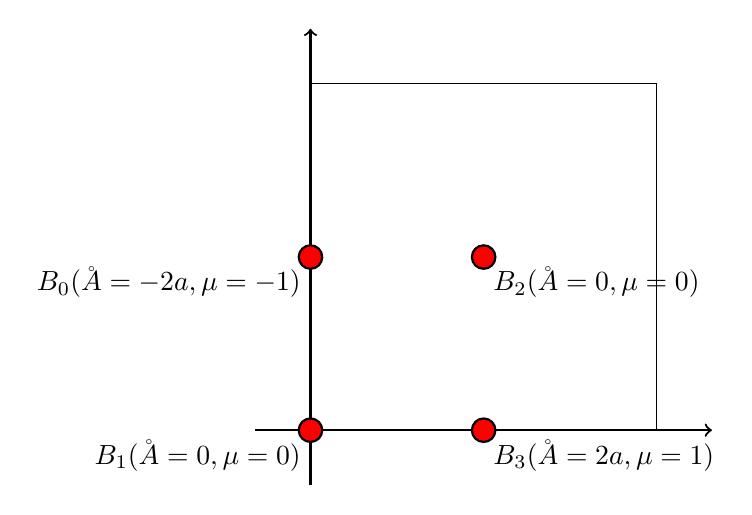
\begin{tikzpicture}[scale=0.7, vertex/.style={draw,circle,thick,fill=red,inner sep=3pt}]
\draw[->,thick] (-1,0) -- (2*pi+1,0);
\draw[->,thick] (0,-1) -- (0,2*pi+1);
\draw (0,0) rectangle (2*pi,2*pi);

\draw (0,0) node[vertex] {} node[below left] {$B_1 (\AA = 0, \mu = 0)$};
\draw (0,pi) node[vertex] {} node[below left] {$B_0 (\AA = -2a, \mu = -1)$};
\draw (pi,0) node[vertex] {} node[below right] {$B_3 (\AA = 2a, \mu = 1)$};
\draw (pi,pi) node[vertex] {} node[below right] {$B_2 (\AA = 0, \mu = 0)$};
\end{tikzpicture}
\caption{The periodic orbits of $H_1$ and their actions and Maslov indices}
\label{orbitsh1}
\end{figure}

Consequently, the vector spaces of the Floer complex are given by
\begin{equation}
\begin{gathered}
\CF_{-1}^\lambda(H_1) = \begin{cases}
0, & \lambda \leq -2a,\\
\braket{B_0} & \lambda > -2a,
\end{cases}
\\
\CF_{0}^\lambda(H_1) = \begin{cases}
0, & \lambda \leq 0,\\
\braket{B_1,B_2} & \lambda > 0,
\end{cases}
\\
\CF_{1}^\lambda(H_1) = \begin{cases}
0, & \lambda \leq 2a,\\
\braket{B_3} & \lambda  > 2a.
\end{cases}
\end{gathered}
\end{equation}

This information can be sumarily represented via the following barcode.
\begin{figure}[H]
\centering
\begin{tikzpicture}
\draw[->,thick] (-4.500,0.000)--(4.500,0.000);
\draw[] (0.000,-0.200)--(0.000,0.200) node[above] {0};
\draw[] (2.500,-0.200)--(2.500,0.200) node[above] {$2a$};
\draw[] (-2.500,-0.200)--(-2.500,0.200) node[above] {$-2a$};
\draw[(-,thick] (-2.500,-0.500)--(4.200,-0.500) node[right] {$B_0$};
\node[] at (5.500,-0.500) {$(\CF_{-1})$};
\draw[(-,thick] (0.000,-1.100)--(4.200,-1.100) node[right] {$B_1$};
\draw[(-,thick] (0.000,-1.500)--(4.200,-1.500) node[right] {$B_2$};
\node[] at (5.500,-1.300) {$(\CF_0)$};
\draw[(-,thick] (2.500,-2.100)--(4.200,-2.100) node[right] {$B_3$};
\node[] at (5.500,-2.100) {$(\CF_1)$};
\end{tikzpicture}
\caption{The barcode of the filtered Floer complex of $H_1$}
\end{figure}
\end{prop}

\section{The Boundary Maps and Symmetries}\label{sec:symmetries}

Now that we have computed the vector spaces of the filtered Floer complex associated to $H_1$, all that remains is to compute the boundary maps. In principle, these depend on a choice of almost-complex structure $J$, which in the case of the torus can be chosen to be the one associated to the usual Riemannian metric, i.e.
\begin{equation}
J(\partial_x) = \partial_y, \quad J(\partial_y) = \partial_x.
\end{equation}

We begin by recalling the definition of $\partial(b)$, where $b$ is a periodic orbit of $H_1$. First, one must compute the Maslov index $\mu(b)$. Then, $\partial(b)$ will be of the form
\begin{equation}
\partial(b) = \sum n(b,c) c,
\end{equation}
where the sum is taken over orbits $c$ whose Maslov index is $\mu(c) = \mu(b)-1$. We will go back to the definition of $n(b,c) \in \Z_2$ shortly, but we remark that this information, together with the fact that Floer homology coincides with Morse homology, is sufficient to compute the boundary maps.

\begin{prop}
The boundary maps of the filtered Floer complex of $H_1$ are null.
\end{prop}

\begin{proof}
It is known that Floer homology coincides with Morse homology, up to a shift in index. Furthermore, every periodic orbit of $H_1$ has action less than, say, $3a$, so the filtered Floer homology of $H_1$ with parameter $\lambda = 3a$ coincides with the Morse homology of the torus, which is known to be $\Z_2, \Z_2^2, \Z_2, 0, 0, \dots$, in degrees $0$, $1$, etc.

Since the dimension of the spaces of the Floer complex of $H_1$ have dimensions $1$, $2$, and $1$ in the appropriate degrees, and 0 in the rest, the boundary maps must be zero, otherwise some dimensions would be lost in taking the quotient for computing the homology.
\end{proof}

Note: The preceding argument does not actually rely on the underlying field, so it would also work for homology taken in other fields. However, we have not defined the Floer homology for fields other than $\Z_2$, so we refrain from generalizing.

In principle, we could end this section here, as we have full information about the Floer complex. However, in order to introduce a concept that will be used in the more complicated example of section \ref{chap:secondexample}, we present an alternative proof that the boundary maps are zero.

We recall the definition of the numbers $n(b,c)$ in the definition of $\partial(b) = \sum n(b,c) c$. They are computed by counting how many pseudo-holomorphic curves connect $b$ and $c$. In the case of the torus, with the almost-complex structure $J$ defined above and a Hamiltionian $H$, a pseudo-holomorphic curve is a $C^\infty$ function $(x(t,s), y(t,s))$, $t \in \R / T\Z$, $s \in \R$, satisfying
\begin{equation}\label{pseudoholomorphic}
\begin{cases}
\displaystyle \diffp x s - \diffp y t = \diffp H x(x,y,t),\\[1em]
\displaystyle \diffp y s + \diffp x t = \diffp H y(x,y,t).
\end{cases}
\end{equation}

We say that such a curve $(x,y)$ connects the periodic orbits $b$ and $c$ if the following limits hold in the $C^\infty$ sense
\begin{equation}
\lim_{s \to -\infty} (x,y)(t,s) = b(t), \; \lim_{s \to \infty} (x,y)(t,s) = c(t).
\end{equation}

The set of such solutions, modulo translation of $s$, is denoted $\moduli(b,c)$.

Now, we are only interested in the number of said curves modulo 2, so if we find any symmetries in $\moduli(b,c)$ in the form of an involution $F \colon \moduli(b,c) \to \moduli(b,c)$ we will only need to examine solutions which are symmetrical, i.e. $F(u) = u$. In our case, such involutions will come from well-chosen changes of variable.

For example, suppose we wish to compute $n(B_3, B_1)$ (see figure \ref{orbitsh1}). The key is the axis of symmetry of the torus about the vertical line $x = \pi$. In other words, if $(x,y)(t,s)$ is a pseudo-holomorphic orbit connecting $B_3$ to $B_1$, i.e. an orbit of $\moduli(B_3,B_1)$, it is reasonable to conjecture that the orbit $(2\pi-x, y)(t,s) = (-x,y)(t,s)$ is also in $\moduli(B_3,B_1)$.

The first thing that needs to be checked is that the $C^\infty$ limits as $s \to \pm \infty$ still coincide with $B_1$ and $B_3$. This is a trivial check, as the reflection about $x = \pi$ preserves the $C^\infty$ norm, as well as the orbits $B_1$ and $B_3$. Therefore, it suffices to check the pseudo-holomorphicity of the orbit $(-x,y)(t,s)$. Unfortunately, this is where we run into problems, because, in general,
\begin{equation}
\label{nottrue1}
\begin{cases}
\displaystyle \diffp{(-x)} s - \diffp y t = \diffp H x(-x,y,t),\\[1em]
\displaystyle \diffp y s + \diffp{(-x)} t = \diffp H y(-x,y,t)
\end{cases}
\text{ is \emph{not} true!}
\end{equation}

In order to correct and prove a statement similar to \eqref{nottrue1}, it is first useful to consider what can be said about $\grad_{x,y} H(x,y,t)$. To do so, we investigate symmetries of $H_t$ in space (and eventually in time) and see how they are reflected in symmetries of $\grad_{x,y} H$.

For example, the Hamiltonian $H_0(x,y,t)$, (as well as its smoothing $H_1$, if it is done with a symmetrical bump function), satisfies the symmetry
\begin{equation}
H(-x,y,t) = H(x,y,t).
\end{equation}

Consequently, taking partial derivatives, we obtain the symmetries
\begin{equation}\label{eq:symmetries1}
- \diffp H x(-x,y,t) = \diffp H x(x,y,t),\quad \diffp H y(-x,y,t) = \diffp H y (x,y,t).
\end{equation}

This points to how \eqref{nottrue1} might be fixed. For example, the right-hand side of the second equation of \eqref{nottrue1} equals
\begin{equation}
\diffp H y (-x,y,t) = \diffp H y (x,y,t) \stackrel{\text{$(x,y)$ pseudo-holom.}}{=} \diffp y s + \diffp{x} t,
\end{equation}
and the last term is not equal to $\diffp y s + \diffp{(-x)} t$ by a factor of $-1$ in the second term. An easy way to correct this factor is to swap the variable $t$ for $-t$. This creates another problem, because $H(-x,y,-t) \neq H(x,y,t)$, but a translation in time yields the symmetry
\begin{equation}
H(-x,y,a - t) = H(x,y,t).
\end{equation}

Therefore, \eqref{eq:symmetries1} can be modified to yield the slightly different symmetries
\begin{equation}
- \diffp H x(-x,y,a-t) = \diffp H x(x,y,t),\quad \diffp H y(-x,y,a-t) = \diffp H y (x,y,t).
\end{equation}

This finally allows us to define the involution. Given an orbit $(x,y)(t,s) \in \moduli(B_3,B_1)$, define
\begin{equation}
(\tilde x, \tilde y)(t,s) = (-x,y)(a-t,s).
\end{equation}

We verify that $(\tilde x, \tilde y) \in \moduli(B_3, B_1)$.
\begin{itemize}
\item The conditions at infinity are verified because the operator $(x,y)(t) \mapsto (-x,y)(a-t)$ preserves $C^\infty$ norm and the constant orbits $B_3$ and $B_1$.

\item The curve $(\tilde x, \tilde y)$ is pseudo-holomorphic, as can be checked directly. As an example, we verify the first equation in \eqref{pseudoholomorphic}; the second equation is verified analogously.

\begin{equation}
\begin{aligned}
\diffp{\tilde x}s - \diffp{\tilde y}t &= \diffp{(-x)(a-t,s)}s - \diffp{y(a-t,s)}t\\
&= - \diffp x s(a-t, s) + \diffp y t(a-t, s)\\
&= - \diffp H x (x(a-t,s), y(a-t,s), a-t)\\
&= \diffp H x (\tilde x(t, s), \tilde y(t, s), t).
\end{aligned}
\end{equation}
\end{itemize}

This proves that the involution $(x,y) \mapsto (\tilde x, \tilde y)$ maps elements of $\moduli(B_3,B_1)$ to itself, so modulo 2 we need only count solutions which are symmetric with regard to this involution. We will now show that there are no such solutions.

If $(x,y) = (\tilde x, \tilde y)$, note that $x(\tfrac a 2, s) = - x(\tfrac a 2, s)$ in the torus, i.e. modulo $2\pi$. Therefore,
\begin{equation}
x(\tfrac a 2, s) \in \{0,\pi\}, \mod 2\pi.
\end{equation}

Now, as $s \to -\infty$ this quantity must converge to $\pi$ and as $s \to \infty$ this quantity converges to $0$. This is a contradiction, because the space of possible values in which $x(\tfrac a 2, s)$ may be in is discrete, and since this quantity is continuous in $s$ it must be constant. Therefore, there are no symmetric solutions, and $n(B_3, B_1) = 0$.

The same symmetry shows that $n(B_2, B_0) = 0$, and a similar argument with the variable change
\begin{equation}
x \to x, y \to -y, t \to a-t,
\end{equation}
shows that the other values of $n$ are also null. This completes the proof of

\begin{prop}
The boundary maps of the filtered Floer complex of $H_1$ are all null. Consequently, the barcode of its time-$2a$ flow coincides with the barcode of the Floer complex of $H_1$, which is represented in the following figure.

\begin{figure}[H]
\centering
\begin{tikzpicture}
\draw[->,thick] (-4.500,0.000)--(4.500,0.000);
\draw[] (0.000,-0.200)--(0.000,0.200) node[above] {0};
\draw[] (2.500,-0.200)--(2.500,0.200) node[above] {$2a$};
\draw[] (-2.500,-0.200)--(-2.500,0.200) node[above] {$-2a$};
\draw[(-,thick] (-2.500,-0.500)--(4.200,-0.500) node[right] {$B_0$};
\node[] at (5.500,-0.500) {$(\HF_{-1})$};
\draw[(-,thick] (0.000,-1.100)--(4.200,-1.100) node[right] {$B_1$};
\draw[(-,thick] (0.000,-1.500)--(4.200,-1.500) node[right] {$B_2$};
\node[] at (5.500,-1.300) {$(\HF_0)$};
\draw[(-,thick] (2.500,-2.100)--(4.200,-2.100) node[right] {$B_3$};
\node[] at (5.500,-2.100) {$(\HF_1)$};
\end{tikzpicture}
\caption{The barcode of the time-$2a$ flow of $H_1$.}
\end{figure}

\end{prop}